\documentclass[a4paper]{article}

\usepackage[english]{babel}
\usepackage[utf8]{inputenc}
\usepackage{amsmath}
\usepackage{minted}
\usepackage{graphicx}

\usepackage[colorinlistoftodos]{todonotes}

\title{DNS Cache Poisoning Attack}


\author{Federica Consoli - 1538420}

\date{\today}

\begin{document}
\maketitle

\begin{abstract}
	The goal of the assignment was to simulate a DNS Cache Poisoning attack. In this report I will discuss the steps taken to prepare for the hack, how it was implemented and what results were obtained.
\end{abstract}

\section{Getting started}
\label{sec:q1}
	The idea behind this hack is to make the DNS accept a specially forged packet. By design, a DNS accepts a response packet only if it matches one of its pending queries. For this to happen, the following conditions need to be satisfied:
	\begin{itemize}
		\item the response arrives on the same UDP port it was sent from
		\item the response's query ID matches the one of the pending query
		\item the response's question section matches the one of the pending query
	\end{itemize}
	The first step is, of course, to obtain the query id and the source port from the DNS server.
	\\\\
	In order to obtain these two information, I decided to use two sockets: one to query the DNS server and one to obtain its answer. The first sockets connects to the IP address of the DNS server on port 53, while the second one is listening on the same port, only this time on my machine. \\I then crafted a query packet for the DNS, asking it to lookup the address for \texttt{badguy.ru} (which corresponds to my machine's address), and sent it to the DNS server via the first socket: within milliseconds, I received the information I needed on the second socket.\\
	\begin{figure}
		\centering
		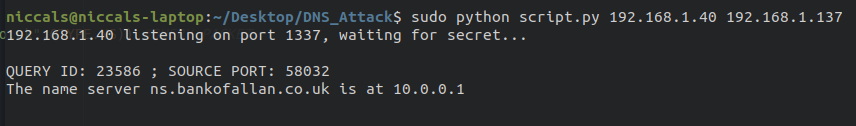
\includegraphics[width=1\linewidth]{qid_srcport}
		\caption[]{First steps}
		\label{fig:qidsrcport}
	\end{figure}
	\\Using a similar approach, I queried the DNS server for the IP address and the hostname of the name server responsible for the victim's domain. This step is necessary because the source ip for the forged DNS responses needs to be spoofed, or else the response would not be accepted by the DNS, since it is not coming from an authoritative server for the targeted domain.
	Once I obtained the IP address, I added it as a static address for one of my machine's interfaces using the command \texttt{ip addr add 10.0.0.1 dev lo}, which later allowed me to perform the spoofing.
	\\\\I then proceeded to configure the file \texttt{config.json} on my virtual machine as shown below. Finally, I connected the VM to my laptop using a bridged network adapter.\\
	\begin{figure}[H]
		\centering
		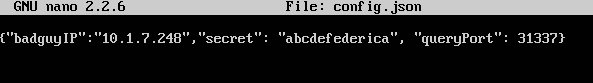
\includegraphics[width=1\linewidth]{config_json}
		\caption{the VM configuration file}
		\label{fig:configjson}
	\end{figure}
	
\section{Implementation}
	The attack was implemented in Python, using the \texttt{dnslib} library, which allowed me to easily create and manipulate DNS packets. The program is launched via \texttt{sudo python bad\_guy\_IP target\_IP}, where \texttt{bad\_guy\_IP} is the attacker's IP addres (namely, my own machine's), while \texttt{target\_IP} represents the IP of the target (the VM).\\
	\\After checking if the arguments are correct, the program spawns two concurring threads, with two different target function: \texttt{poison} and \texttt{listen}.\\
	\\The \texttt{poison} function is the one that actually implements the attack. As mentioned before, this function uses two functions (\texttt{get\_qid\_and\_port} and \texttt{get\_ns}) to retrieve the information needed to carry out the attack, namely the query ID, the source port of the DNS, the IP and the hostname of the target's name server.\\
	\\After this, the program creates a socket for UDP traffic and binds it to the IP address obtained from \texttt{get\_ns} (which was previously added to my \texttt{lo} interface). It then queries the DNS for the address of the domain \texttt{random.bankofallan.co.uk} and starts flooding the server with response packets.
	\begin{figure}[H]
		\centering
		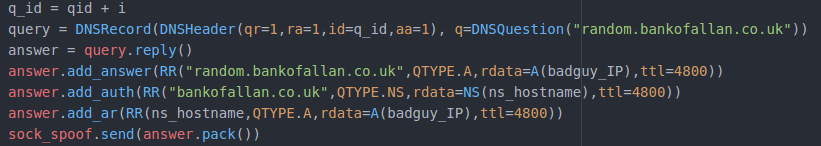
\includegraphics[width=1\linewidth]{response_flooding}
		\caption{Response structure}
		\label{fig:responseflooding}
	\end{figure}
	From the code snippet above, we can notice the following:
	\begin{enumerate}
		\item the \textit{query ID} is incremented at each iteration, to try and match the query ID generated from the DNS server (which is randomly incremented)
		\item the \textit{answer} section contains the resolution for the requested domain, with an IP address of choice (in a real attack, this would be the address of the attacker's web server).
		\item the \textit{authority} section contains the hostname for the authoritative name server for \texttt{bankofallan.co.uk}, which was previously retrieved with the function \texttt{get\_ns}. However, in the \textit{additional record} section, the name server is linked to an IP chosen by the attacker: this means that after a successful poisoning, the attacker will become the owner of the whole zone.
	\end{enumerate}
	\begin{figure}[H]
		\centering
		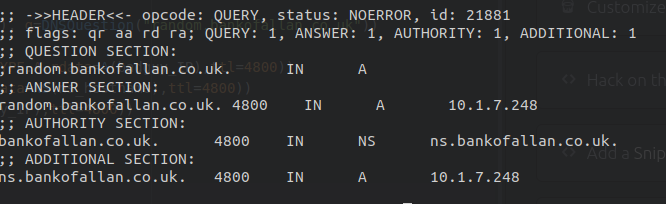
\includegraphics[width=1\linewidth]{forged_response}
		\caption{The forged response}
		\label{fig:forgedresponse}
	\end{figure}
	The \texttt{listen} function, on the other hand, creates a socket listening on port 1337. This is where the \textit{secret} is received, which indicates that the cache was successfully poisoned. When the secret is received, it is simply printed by the function.
\section{The secret}
	As mentioned before, when I succeeded in carrying out the attack I received a \textit{secret} on port 1337: what I received was the hash of the string I inserted in the field "secret" in the \texttt{config.json} file, as shown in Figure \ref{fig:configjson}.

\end{document}